\documentclass[sigconf,anonymous,review]{acmart}
\setcopyright{none}
\setlength{\emergencystretch}{2em}
\settopmatter{printacmref=false}
\renewcommand\footnotetextcopyrightpermission[1]{}
\acmConference[IAFM '26]{Workshop on Interpretability and Alignment of Financial Models}{November 2026}{Milan, Italy}
\acmYear{2026}
\title{When Portfolio Rewards Miss the Target: Exact Mismatch and Policy Alignment}
\author{Anonymous Author(s)}
\newcommand{\E}{\mathbb{E}}
\newcommand{\Var}{\operatorname{Var}}
\newcommand{\Cov}{\operatorname{Cov}}
\newcommand{\eq}{\mathrm{eq}}
\newtheorem{proposition}{Proposition}
\newtheorem{theorem}{Theorem}
\begin{document}
\begin{abstract}
A portfolio reward can be optimised accurately while implementing a different financial preference. We quantify this difference for terminal mean--variance equilibrium and for constrained allocation with trading costs. In the independent-return benchmark, an exact leading discrepancy remains after the best scalar calibration of a quadratic wealth-increment reward. For fitted allocation, jointly scaling risk and deterministic costs through the mean--variance auxiliary identity preserves the reference; we bound imperfect calibration and optimisation. Historical tests cross six covariance estimators with 10, 30 and 49 US industry portfolios over 432 months. Data-driven linear shrinkage and observed-factor estimates change the reference policy, but joint calibration preserves alignment within every model. Unconstrained scalar calibration worsens alignment in all twelve larger-universe cases. One existing MVPI update, initialised from holdings, reduces mean allocation error by 97.8--98.6\% without supplying the reference. Known-covariance simulations and a borrowing/shorting example separate estimation error from reward error. Realised results do not establish investment superiority. The contribution is a quantitative audit of the preference implemented by a portfolio reward, with corrections and independently checked error budgets.
\end{abstract}
\ccsdesc[500]{Computing methodologies~Reinforcement learning}
\ccsdesc[300]{Applied computing~Economics}
\keywords{portfolio allocation, reward alignment, covariance estimation, mean--variance, model validation}
\maketitle

\section{Introduction}
A portfolio mandate specifies a trade-off between return, risk and costs. A learning algorithm acts on a reward. These descriptions need not select the same allocation: a second-moment penalty also penalises squared expected return, while correcting risk alone can change the effective preference over trading costs. Better optimisation can therefore implement the wrong mandate more accurately. Kolm and Ritter~\cite{kolm2025}, pp. 90--91, explicitly call for rewards that reflect investment mandates. We ask how to test this correspondence, rather than infer it from the reward's name or a favourable backtest.

This question is distinct from estimation risk. Markowitz~\cite{markowitz1952} separates beliefs about returns from decisions made using those beliefs; DeMiguel et al.~\cite{demiguel2009} show how estimation error can overwhelm the gains from optimal diversification. Shrinkage and factor models improve or regularise inputs. Reward calibration concerns the decision conditional on those inputs. Confounding the two can make an estimator change look like a reward failure, or a favourable backtest look like proof of alignment.

We compare the intended policy, the exact reward-induced policy and its numerical approximation. Our theoretical result gives the exact leading discrepancy remaining after optimal scalar tuning in a terminal-equilibrium benchmark. For constrained fitted allocation, we build on the established mean auxiliary~\cite{zhang2021}, identify cost distortion, and bound the effect of an imperfect calibration anchor. A factorial historical audit changes covariance models and rewards separately. Simulations with known covariance identify estimation error directly; historical investment results remain a separate test. The resulting explanation is operational: specify the preference, identify the decision change, and verify whether a particular correction removes it.

\section{Related work and comparison design}
\paragraph{Financial estimation and costs.}
DeMiguel, Garlappi and Uppal~\cite{demiguel2009}, Tables 3--5, compare fourteen allocation models with $1/N$ using Sharpe, certainty-equivalent return and turnover. Their Proposition 1 and Figure 1 relate estimation requirements to dimension and investment opportunities; they do not prescribe a minimum portfolio size. Table 2 includes ten industries plus the market. We retain this compact benchmark and test finer industry classifications.

Ledoit and Wolf's linear estimators shrink toward a scaled identity~\cite{ledoit2004identity}, Section 3.3, or constant correlation~\cite{ledoit2004correlation}, Appendices A--B of the inspected working paper. Fan et al.~\cite{fan2008}, Section 2, Eq. (4), estimate covariance from observed factors and residual variances. We implement these constructions with explicit finite-sample conventions. The nonlinear estimator of Ledoit and Wolf~\cite{ledoit2017}, Section 4.3/Table 1, is a further input-estimation approach, not a method reproduced here.

G\^arleanu and Pedersen~\cite{garleanu2013}, Eq. (4) and Propositions 2--3, derive a dynamic policy with predictable returns and quadratic trading costs. DeMiguel, Mart\'in-Utrera and Uppal~\cite{demiguel2024}, Eq. (6) and Tables II--III, study cost-aware conditional multifactor allocation. These are positive examples of explicit financial objectives. Our rolling one-period L1-cost target is a different object, not a replication of either strategy.

\paragraph{Financial learning and reward choices.}
Kolm and Ritter~\cite{kolm2025}, pp. 90--92 and Exhibit 3, identify reward design, interpretability and validation as practical obstacles and recommend hybrid classical/RL models. Their Exhibit 2 (p. 84) places reward specification before agent training; we make the intervening mandate-alignment test quantitative. Their article is an equation-free overview (p. 82), with no new empirical strategy to reproduce. Its discussion of known-policy comparisons (p. 87) also precludes treating benchmark validation itself as new.

Their earlier hedging paper~\cite{kolm2019}, Eqs. (8)--(10), explicitly treats a quadratic increment reward as an approximation. Jiang et al.~\cite{jiang2025}, Eq. (8), combine log return and variance; their 2024 paper~\cite{jiang2024}, Eq. (4), combines portfolio value, variance and costs. Habibnia and Soltanzadeh~\cite{habibnia2024}, Eq. (8)/Table 2, use an asymmetric PnL reward with SAC, shorting and lending. Our common-environment adaptations isolate these preferences; they do not reproduce the published architectures or markets.

Direct preference optimisation and known-policy validation already exist. Simon et al.~\cite{simon2026}, Eq. (17), use centred MV utility; Gollart and Okhrin~\cite{gollart2025}, Section 4.2.1/Table 1, compare learned terminal-utility policies with an analytical benchmark, as does related control work~\cite{chaouki2020}. Cong et al.~\cite{cong2026}, Eqs. (19)--(20), allow differentiable trajectory objectives including Sharpe. A different objective is not inherently a defective one.

\paragraph{Time consistency and transformations.}
Precommitment~\cite{ling2000} and equilibrium~\cite{basak2010,dai2023} answer different questions. Czichowsky~\cite{czichowsky2013}, Lemma 3.2 of the inspected preprint, includes a hedge against continuation covariance. Bj\"ork et al.~\cite{bkm2016}, Propositions 8.1 and 10.2 of the long preprint, develop equivalent objectives and terminal-unit variance penalisation. MVPI~\cite{zhang2021} supplies the mean auxiliary used below. Our theoretical increment is the exact leading minimum discrepancy for the specified raw-reward family, not a new equivalent-objective method.

\section{An exact test of terminal-objective alignment}
\subsection{Market, reference and discrepancy}
Consider independent excess returns $P_t\in\mathbb R^n$ with constant mean $m\ne0$ and positive definite covariance $\Sigma$. Wealth evolves as
\begin{equation}
 X_{t+1}=sX_t+P_t^\top u_t,\qquad X_0=x_0,
\end{equation}
with unrestricted risky dollar positions $u_t$ and constant gross risk-free return $s>0$. The terminal objective is $J=\E X_T-\varphi\Var X_T$, $\varphi>0$. The time-consistent equilibrium policy is
\begin{equation}
 u_t^\eq=\frac{\Sigma^{-1}m}{2\varphi H_t},\qquad H_t=s^{T-t-1}.
\end{equation}
It is not the initial-date precommitment maximiser. Define $M=\Sigma+mm^\top$, $d=M^{-1}m$, $\nu=m^\top d<1$ and $b=[2\varphi(1-\nu)]^{-1}$. The reward family is $r_t=\Delta X_t-\kappa(\Delta X_t)^2$, with one constant $\kappa>0$. Let $\pi^\kappa$ be its exact additive-reward optimum, and measure
\begin{equation}
 D^2=\sum_{t=0}^{T-1}\E_{\pi^\kappa}\|\pi^\kappa(t,X_t)-u_t^\eq\|^2.
\end{equation}
This is an occupancy-dependent discrepancy, not a symmetric policy metric.

\subsection{What scalar calibration cannot repair}
\begin{theorem}\label{th:mismatch}
For fixed $T\ge2$, as $s\to1$,
\begin{align}
 \min_{\kappa>0}D&=c_T|s-1|+O((s-1)^2),\\
 c_T&=\|d\|b\sqrt{\frac{T(T^2-1)}3+\frac{\nu(1-\nu)T(T-1)}2}.
\end{align}
At $s=1$ exact matching holds for $\kappa=\varphi(1-\nu)$. For $s\ne1$, $T\ge2$, exact matching along the surrogate occupancy is impossible.
\end{theorem}
\begin{proof}
Write the Bellman value $W_t(x)=p_tx^2+q_tx+c_t$, with $p_T=q_T=0$ and $g_t=\kappa(s-1)-sp_{t+1}$. Completing the square gives $u_t=\alpha_tx+\beta_t$ and
\begin{align}
 \alpha_t&=-\frac{dg_t}{\kappa-p_{t+1}},&
 \beta_t&=\frac{d(1+q_{t+1})}{2(\kappa-p_{t+1})},\\
 p_t&=\frac{\kappa p_{t+1}-(1-\nu)g_t^2}{\kappa-p_{t+1}},&
 1+q_t&=(1+q_{t+1})\left(s-\frac{\nu g_t}{\kappa-p_{t+1}}\right).
\end{align}
Induction gives $p_t\le0$, so the action Hessian is negative definite and these are global Markov optima. Set $e=s-1$, $h=(2\kappa)^{-1}$. The ratios $p_t/\kappa$ and $q_t$ are independent of $\kappa$, hence pathwise $X_t=L_t(e)x_0+hZ_t(e)$. Consequently $D^2=F(e,h)$ is exactly quadratic in $h$, with analytic coefficients near zero and $F(0,h)=T\|d\|^2(h-b)^2$. Its global minimiser is analytic and remains positive near zero.

Put $\kappa=\varphi(1-\nu)(1+we)$. The leading action difference is $de$ times
\[
 -X_t+b[(T-t-1)(2-\nu)-w].
\]
At $e=0$, $\E X_t=x_0+t\nu b$ and $\Var X_t=tb^2\nu(1-\nu)$. Minimisation yields $w^*=(T-1)(1-\nu)-x_0/b$. The centred means are $b(T-1-2t)$; summing their squares and variances gives the displayed $c_T^2$. Analyticity then gives the stated remainder after taking square roots.

Finally, matching at the first date forces a nonzero equilibrium action and positive subsequent wealth variance. At the final date the surrogate has slope $-d(s-1)$ whereas equilibrium is constant. Almost-sure equality is impossible when $s\ne1$.
\end{proof}
The coefficient grows as $T^{3/2}$ for large $T$, but the expansion is for fixed $T$; no uniform joint interest--horizon limit is claimed. The obstruction concerns this reward family, not all additive objectives.

\subsection{A reference-preserving reward}
Allow moments to vary by date while returns remain independent. Define $Y_t=H_tP_t^\top u_t$ and use
\begin{equation}\label{eq:design}
 r_t^{\rm design}=Y_t-\varphi(1-\nu_t)Y_t^2.
\end{equation}
The expected reward is strictly concave. Its maximiser is
\[u_t=\frac{\Sigma_t^{-1}m_t}{2\varphi H_t}.\] Future rewards admit state-independent maximisers, so backward induction recovers the equilibrium. This construction specialises the equivalent-objective approach of Bj\"ork et al.\ \cite{bkm2016} and changes the optimum of the original raw reward. Dependent returns require continuation terms, so Eq.\ \eqref{eq:design} is not applied as a historical multiperiod theorem.

\begin{figure}[t]
\centering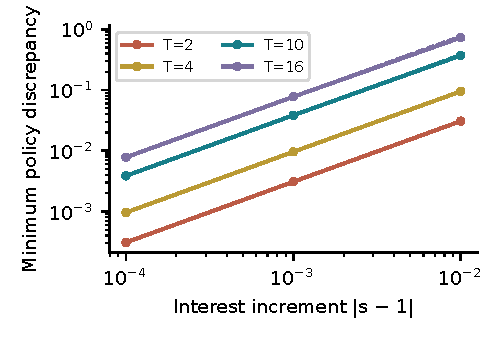
\includegraphics[width=\columnwidth]{figures/theory.pdf}
\caption{Exact minimum discrepancy (points and solid lines) and local prediction $c_T|s-1|$ (dashed lines). Here $x_0=\varphi=1$, $m=(.06,.04,.02)$, volatilities $(.18,.12,.08)$, and correlations $(\rho_{12},\rho_{13},\rho_{23})=(.30,-.10,.05)$. This concerns terminal equilibrium, not the fitted historical reference.}
\Description{Log-log plot comparing exact discrepancy with the local formula for four horizons.}
\label{fig:theory}
\end{figure}

\section{Constrained alignment with turnover costs}
Historical implementation adds constraints and costs. On a fixed past-only estimated state, let $C$ be the simplex, $p$ the pre-trade allocation and $c(u)=\|u-p\|_1$. Define the fitted one-period preference
\begin{equation}\label{eq:target}
 F(u)=m^\top u-\varphi u^\top\Sigma u-\lambda c(u),\quad u\in C.
\end{equation}
Its unique optimum $u^*$ is a \emph{fitted reference}, not the unknown true market optimum. This section does not extend Theorem~\ref{th:mismatch} to estimated or dependent markets.

\begin{proposition}\label{prop:joint}
Let $y^*=m^\top u^*$ and $A=1+2\varphi y^*>0$. The second-moment reward objective
\begin{equation}
 Q(u)=m^\top u-\frac{\varphi}{A}u^\top M u-\frac{\lambda}{A}c(u)
\end{equation}
has the same unique maximiser as $F$.
\end{proposition}
\begin{proof}
For all feasible $u$,
\begin{equation}\label{eq:identity}
 AQ(u)=F(u)-\varphi(m^\top u-y^*)^2+\varphi(y^*)^2.
\end{equation}
At $u^*$ the square vanishes and $F$ is maximal. Since $A>0$, the assertion follows.
\end{proof}
The argument applies to any feasible set with a global maximiser. Convexity and positive definite covariance ensure uniqueness here. The identity follows the mean auxiliary used in MVPI\ \cite{zhang2021}.

If only the risk coefficient is divided by $A$, while the cost coefficient stays $\lambda$, the right-hand side of Eq.\ \eqref{eq:identity} gains the extra term
\begin{equation}\label{eq:costdistortion}
 -2\varphi y^*\lambda c(u).
\end{equation}
When $y^*>0$, this increases the effective cost preference. It need not imply monotone realised turnover on the strategy's evolving path. The unconstrained formula $\varphi(1-\nu)$ likewise need not calibrate a constrained optimum.

Joint calibration uses $u^*$ and therefore serves as a certificate of alignment with a known reference. As a constructive prior-art comparator, we also alternate maximising
\begin{equation}
 (1+2\varphi y)m^\top u-\varphi u^\top Mu-\lambda c(u)
\end{equation}
and setting $y=m^\top u$. This is an adaptation of the MVPI mean auxiliary to the constrained one-period problem. Including the term $-\varphi y^2$ gives a jointly strictly concave objective, since its quadratic block has Schur complement $\Sigma\succ0$. Exact block updates converge to the same target. This provides a constructive comparator with the same optimum.


\subsection{Imperfect anchors and other deterministic costs}
Replace $\lambda c(u)$ by any convex deterministic cost $g(u)$, including borrowing spreads and short-position charges, on a convex feasible set. For an anchor $a$, set $A_a=1+2\varphi a>0$ and
\[
Q_a(u)=m^\top u-\frac{\varphi}{A_a}u^\top Mu-\frac{g(u)}{A_a}.
\]
If $\widehat u$ is $\epsilon$-optimal for $Q_a$, the same auxiliary identity yields
\begin{align}\label{eq:budget}
0\le F(u^*)-F(\widehat u)
&\le\varphi(y^*-a)^2+A_a\epsilon,\\
\|\widehat u-u^*\|^2
&\le\frac{\varphi(y^*-a)^2+A_a\epsilon}
{\varphi\lambda_{\min}(\Sigma)}.\nonumber
\end{align}
Indeed, compare $Q_a(\widehat u)$ with $Q_a(u^*)$ in Eq.\ \eqref{eq:identity}, retain the anchor $a$, and drop the nonpositive square at $\widehat u$. Strong concavity gives the second bound. These are consequences of the prior identity, not a new general auxiliary algorithm. The value bound survives a singular covariance; the distance bound and uniqueness need not.

Choosing $a=m^\top p$ gives one MVPI portfolio update initialised at current holdings, without supplying the target. It need not be exact, but Eq.\ \eqref{eq:budget} makes its error explicit. A certified approximate reference can bound the unknown $y^*$ (Appendix~\ref{app:bounds}). Every term in $g$ must be scaled: correcting turnover while leaving financing charges unchanged can still alter the mandate.


\section{Historical and controlled experiments}
\subsection{Common information, different covariance models}
We use Kenneth French's value-weighted US industry monthly returns and Fama--French factors~\cite{french}, preserving the archived August 2026 vintage. Estimation data start in 1970; evaluation covers January 1990--December 2025 (432 months). These are revised research portfolios, not point-in-time tradable funds; internal industry-reconstruction costs are unavailable. At each date we use only the previous 120 months. Means are unshrunk sample excess-return means, $\varphi=5$, and $\lambda=0.001$ per unit L1 turnover. Portfolios are long-only and fully invested.

Six covariance specifications are crossed with $N=10,30,49$: sample covariance; the original fixed 10\% diagonal shrinkage; data-driven Ledoit--Wolf identity and constant-correlation shrinkage; and one- and three-observed-factor models. The factors are market excess return, SMB and HML from the same archived source. All estimates use comparable covariance units; factor regressions include an intercept and diagonal residual variances (Appendix~\ref{app:estimators}). Hyperparameters and the primary extension protocol were fixed before inspecting its outcomes.

For reward fidelity, methods share their covariance model's target pre-trade holdings, moments and constraints. For cross-model comparisons, each covariance target is instead evaluated at the original diagonal-model target's holdings. Thus changes in estimated risk are distinguished from changes in reward. Each strategy follows its own holdings for realised performance, paying $\lambda\|u_t-p_t\|_1$ under an explicit first-order cost convention. We report allocation distance, fitted regret, net excess-return MV, excess Sharpe, turnover and drawdown.

\subsection{Published formulations and financial controls}
The methods include the fitted MV target, raw second moment, unconstrained scalar, risk-only and joint calibration, equal weight and cost-aware minimum variance. MVPI and the Jiang log-minus-variance adaptation remain in the ten-industry primary comparison. Log preferences use past monthly total returns with hard simplex constraints and a separate turnover charge; published neural architectures are not reproduced.

For Habibnia and Soltanzadeh~\cite{habibnia2024}, we explicitly restrict Eq. (8) to long-only, unit deployed capital, assetwise monthly PnL, with their loss penalty 25 and cost multiplier $25/5$. Shorts, lending and SAC are not reproduced. Penalties 1 and 5 are sensitivity checks, not selected replacements. This comparator represents a downside preference rather than an intended implementation of MV.

\begin{table*}[t]
\centering
\caption{Ten-industry comparison, 1990--2025. All distances and gaps here use the original fixed-diagonal MV reference at its common states. Covariance rows therefore measure a model change, not pure reward misalignment. Realised metrics use own-state paths. Published formulations are adapted, not complete algorithm replications; bold identifies our exact construction, not superior investment performance.}
\label{tab:historical}
\begin{tabular}{@{}p{.235\textwidth}p{.25\textwidth}rrrr@{}}\toprule
Method & Source / role & \shortstack{Allocation\\distance} & \shortstack{Reference gap\\(bp)} & \shortstack{Excess\\Sharpe} & \shortstack{Realised MV\\(bp)}\\\midrule
Fitted MV reference & Markowitz (1952) & 0.00000 & 0.0000 & 0.570 & -8.497 \\
Minimum variance & Markowitz (1952) & 0.23843 & 9.0252 & 0.645 & 5.274 \\
MV, LW identity & Ledoit--Wolf (2004) & 0.00538 & 0.0055 & 0.572 & -8.442 \\
MV, LW correlation & Ledoit--Wolf (2004) & 0.02196 & 0.1158 & 0.547 & -11.917 \\
MV, market factor & Fan et al. (2008) & 0.05711 & 1.0487 & 0.585 & -4.738 \\
MV, three factors & Fan et al. (2008) & 0.04881 & 0.6407 & 0.555 & -8.532 \\
Equal weight & DeMiguel et al. (2009) & 0.43495 & 46.2626 & 0.622 & -11.893 \\
Raw second moment & Kolm--Ritter (2019) & 0.00843 & 0.0148 & 0.573 & -7.182 \\
MVPI adaptation & Zhang et al. (2021) & 0.00000 & 0.0000 & 0.570 & -8.497 \\
One MVPI step & Zhang et al. (2021) & 0.00014 & 0.0000 & 0.570 & -8.442 \\
Assetwise PnL, restricted & Habibnia--Soltanzadeh (2024) & 0.79645 & 40.2554 & 0.449 & -23.619 \\
Log minus variance & Jiang et al. (2025) & 0.01286 & 0.0287 & 0.572 & -7.123 \\
MV, sample covariance & Sample control (2026) & 0.01449 & 0.0356 & 0.555 & -10.114 \\
Log utility & Log-utility control (2026) & 0.54848 & 39.7855 & 0.344 & -133.295 \\
Unconstrained scalar & Analytical control (2026) & 0.00540 & 0.0043 & 0.568 & -8.882 \\
Risk-only calibration & Calibration ablation (2026) & 0.00510 & 0.0033 & 0.571 & -8.365 \\
\midrule
\textbf{Joint calibration (ours)} & \textbf{This study (2026)} & \textbf{0.00000} & \textbf{0.0000} & \textbf{0.570} & \textbf{-8.497} \\
\bottomrule\end{tabular}

\par\smallskip
\parbox{\textwidth}{\footnotesize\emph{Sources:} MV foundation~\cite{markowitz1952}; linear shrinkage~\cite{ledoit2004identity,ledoit2004correlation}; factor covariance~\cite{fan2008}; $1/N$~\cite{demiguel2009}; increment reward~\cite{kolm2019}; MVPI~\cite{zhang2021}; restricted PnL~\cite{habibnia2024}; log--variance~\cite{jiang2025}. Control dates denote this implementation.}
\end{table*}

Table~\ref{tab:historical} places the covariance alternatives in the same investment evaluation. A separate within-model comparison is essential: the three-factor target is 0.04881 from the ten-industry diagonal target, but joint calibration agrees with that three-factor target to numerical precision. Treating 0.04881 as reward error would confuse two interventions.

\subsection{Dimension and covariance results}
The ratios $N/L$ are 0.083, 0.250 and 0.408, with 65, 495 and 1,274 distinct mean/covariance entries. DeMiguel et al.'s~\cite{demiguel2009} 3,000/6,000-month examples are model-dependent, not universal thresholds. The industry classifications change the opportunity set as well as dimension; these are overlapping US-market robustness checks, not independent replications or a causal experiment in $N$ alone. They test covariance and reward fidelity, not the large-universe RL scalability discussed by Kolm and Ritter~\cite{kolm2025}, pp. 88 and 90.

\begin{table*}[t]
\centering
\caption{Within-estimator fidelity and own-state performance across all eighteen covariance/universe cases. Distances use each estimator's own fitted reference. Joint calibration agrees with it; minimum variance generally represents a different preference. Monthly MV scores are in basis-point units.}
\label{tab:covariance}
\begin{tabular}{rlrrrrr}\toprule
$N$ & Covariance & Raw distance & Scalar distance & \textbf{Joint (ours)} & \shortstack{Target/joint\\MV (bp)} & \shortstack{Minimum-variance\\MV (bp)}\\\midrule
10 & Sample & 0.00874 & 0.00642 & $\mathbf{1.24\times10^{-8}}$ & -10.114 & 4.600 \\
10 & Fixed diagonal & 0.00843 & 0.00540 & $\mathbf{1.40\times10^{-8}}$ & -8.497 & 5.274 \\
10 & LW identity & 0.00838 & 0.00545 & $\mathbf{8.50\times10^{-9}}$ & -8.442 & 5.513 \\
10 & LW correlation & 0.01034 & 0.00637 & $\mathbf{1.28\times10^{-8}}$ & -11.917 & 2.684 \\
10 & Market factor & 0.00827 & 0.00809 & $\mathbf{7.15\times10^{-9}}$ & -4.738 & 4.783 \\
10 & Three factors & 0.00873 & 0.00653 & $\mathbf{2.84\times10^{-9}}$ & -8.532 & 3.758 \\
\midrule
30 & Sample & 0.01967 & 0.04343 & $\mathbf{5.52\times10^{-8}}$ & -26.902 & -3.284 \\
30 & Fixed diagonal & 0.01852 & 0.02183 & $\mathbf{6.87\times10^{-8}}$ & -26.096 & -0.416 \\
30 & LW identity & 0.01789 & 0.02273 & $\mathbf{9.23\times10^{-8}}$ & -25.583 & -0.025 \\
30 & LW correlation & 0.01889 & 0.02717 & $\mathbf{5.78\times10^{-8}}$ & -26.613 & -3.158 \\
30 & Market factor & 0.01782 & 0.04360 & $\mathbf{7.93\times10^{-8}}$ & -24.766 & 3.947 \\
30 & Three factors & 0.01921 & 0.03129 & $\mathbf{7.02\times10^{-8}}$ & -28.840 & -0.012 \\
\midrule
49 & Sample & 0.02205 & 0.11244 & $\mathbf{1.59\times10^{-7}}$ & -30.077 & -6.492 \\
49 & Fixed diagonal & 0.02079 & 0.05354 & $\mathbf{1.57\times10^{-7}}$ & -30.567 & -4.808 \\
49 & LW identity & 0.02007 & 0.05244 & $\mathbf{1.48\times10^{-7}}$ & -29.570 & -4.062 \\
49 & LW correlation & 0.02232 & 0.06635 & $\mathbf{1.40\times10^{-7}}$ & -32.948 & -5.934 \\
49 & Market factor & 0.02174 & 0.08354 & $\mathbf{1.36\times10^{-7}}$ & -26.680 & 0.190 \\
49 & Three factors & 0.02249 & 0.06158 & $\mathbf{1.19\times10^{-7}}$ & -31.047 & -3.013 \\
\bottomrule\end{tabular}

\end{table*}

Joint mean distances are below $1.60\times10^{-7}$ in every case (Table~\ref{tab:covariance}). Raw distances range from 0.00827 to 0.02249. Unconstrained scalar calibration worsens both distance and fitted regret in all twelve 30/49-industry cases, regardless of covariance estimator. The original seventeen-setting ten-industry grid also preserves joint alignment across risk coefficients, costs, windows and diagonal-shrinkage levels; its largest mean distance is $1.54\times10^{-7}$.

Covariance choice changes realised results without establishing a winner. For example, the market-factor target improves monthly MV over fixed diagonal by 3.758, 1.330 and 3.887 bp for $N=10,30,49$. All fifteen cross-estimator target comparisons have paired 95\% intervals containing zero, as do simultaneous path-bootstrap bands. Minimum variance has the highest realised MV among the quadratic methods in every covariance/universe case. Joint calibration remains below raw in realised MV throughout; correcting the mandate is not a performance guarantee.

\begin{figure*}[t]
\centering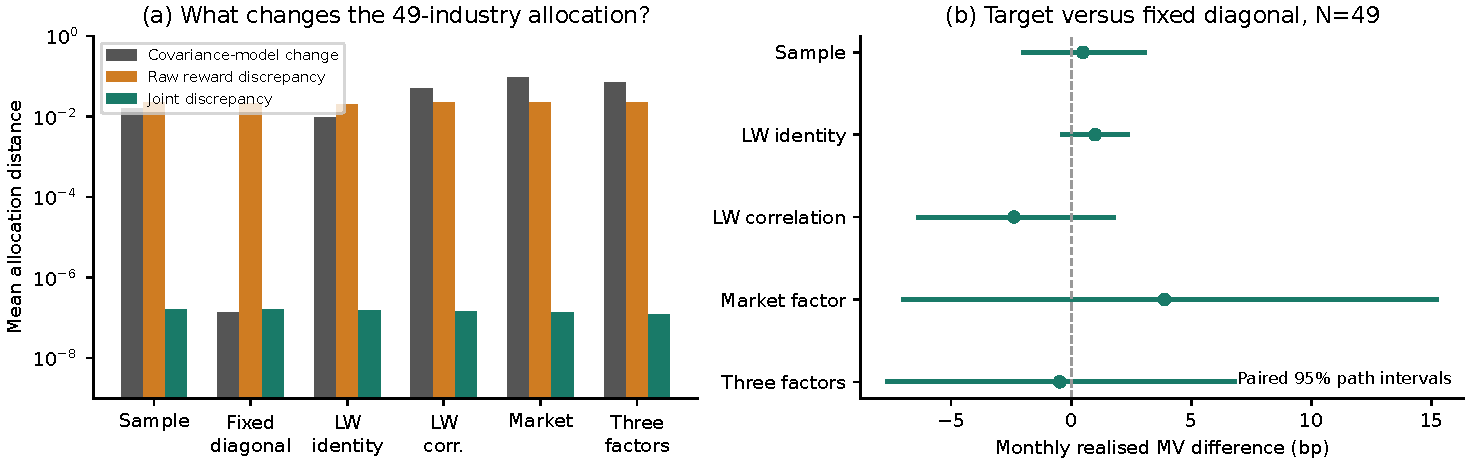
\includegraphics[width=\textwidth]{figures/covariance.pdf}
\caption{Covariance changes and reward changes answer different questions. Left: for 49 industries, model displacement is measured from fixed diagonal at its common states; raw/joint discrepancies are measured within each model. The fixed-diagonal model displacement is zero (display floor $10^{-9}$). Right: paired 95\% intervals for realised target MV differences all cross zero.}
\Description{Log-scale allocation distances and paired confidence intervals for five alternative covariance estimators.}
\label{fig:covariance}
\end{figure*}

\subsection{Known covariance and financing mechanisms}
To identify estimation error directly, we simulate three observed Gaussian factors with either independent residuals or within-block residual correlation 0.4. We cross $N=10,49,100$, $L=60,120$, thirty matched seeds and six estimators: 2,160 fitted problems, including $N>L$. Population means are held known to isolate covariance estimation. The same constrained objective supplies the population reference; no historical forecasting accuracy is inferred.

At $N=100,L=120$, three-factor estimation lowers mean population MV regret from 1.40 to 1.11 bp with independent residuals. With correlated residuals it gives 1.33 versus sample covariance's 1.29 bp; that paired difference is uncertain. A misspecified market-only factor has much larger regret despite remaining compatible with exact reward calibration (Figure~\ref{fig:simulation}). Maximum absolute joint fitted regret across simulations is below $10^{-12}$. Good reward semantics cannot repair a misspecified risk model.

\begin{figure*}[t]
\centering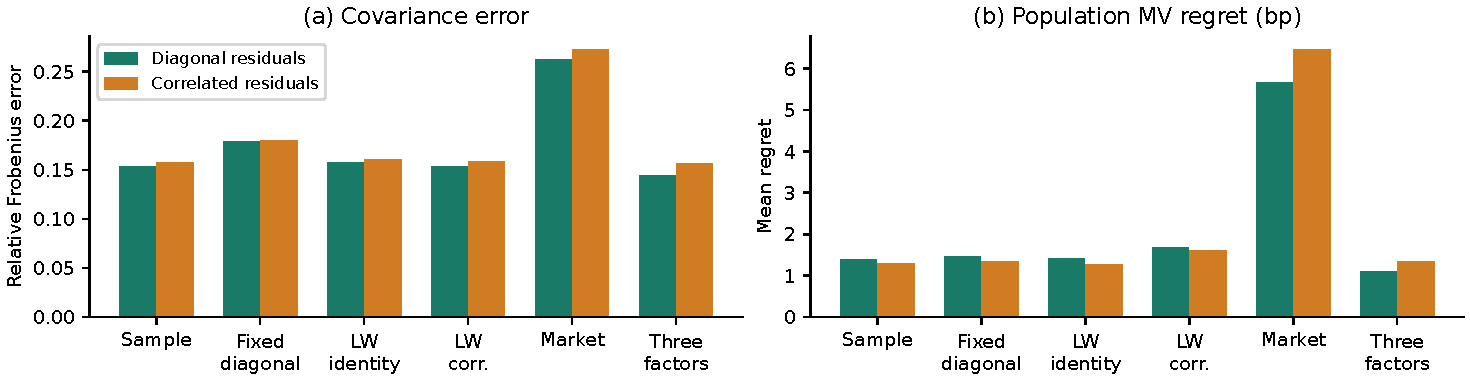
\includegraphics[width=\textwidth]{figures/covariance_simulation.pdf}
\caption{Known-covariance diagnostic, $N=100,L=120$, thirty seeds. Covariance error and population-objective regret are distinct from reward error. Three-factor structure helps when residual independence holds; imposing only one factor misses genuine risks in this design. Bars are descriptive means, not a universal ranking.}
\Description{Two grouped bar charts compare covariance errors and true objective regret under independent and correlated residuals.}
\label{fig:simulation}
\end{figure*}

A separate fifty-state convex example allows short positions, borrowing and a lending/cash position, with deterministic borrowing spreads and short fees. Joint scaling of every cost yields mean allocation discrepancy $1.51\times10^{-7}$; scaling turnover but leaving financing charges unchanged gives 0.00997. This checks the cost mechanism, not the crypto environment of Habibnia and Soltanzadeh.

\section{Numerical accuracy and practical calibration}
Quadratic solutions are checked by an independent linear-programme first-order certificate in original objective units; accepted gaps are at most $2\times10^{-7}$. Reconstruction from original returns and saved weights verifies 58,320 historical decisions, including a sequential exploratory one-step MVPI comparison. Fifty unit tests cover estimator formulas, constraints, calibration, financing and parser boundaries. Covariance shrinkage is checked against an independent library and a direct elementwise fourth-moment calculation.

The one-step method initialises the auxiliary mean from current pre-trade holdings, not the fitted optimum. It was added after the primary covariance results, without tuning, and evaluated in every covariance/universe case. Under fixed diagonal its mean distances are 0.000141, 0.000307 and 0.000343 for $N=10,30,49$, versus raw 0.00843, 0.01852 and 0.02079. Across all eighteen cases, the reduction is 97.8--98.6\%. It reduces alignment error with one existing MVPI update; it is neither a new iterative algorithm nor evidence of investment superiority. The approximate-anchor bounds hold on 144 separately saved January checks for the 49-industry identity-shrinkage and three-factor models.

Optimisation remains a separate issue. The earlier five-seed experiment optimises independent softmax logits on each of 432 fitted states at 50, 250, 1,000 and 5,000 Adam steps. It diagnoses finite-budget error, not predictive generalisation. For an exact reward optimum $u_r$ and a learned approximation $\widehat u_r$,
\[
F(u^*)-F(\widehat u_r)=
[F(u^*)-F(u_r)]+[F(u_r)-F(\widehat u_r)].
\]
The second term is signed and differs from the nonnegative own-reward optimisation gap. Better raw-reward optimisation cannot remove the exact design discrepancy; equivalent limiting policies can still have different finite-budget trajectories.

\section{Financial semantics and model validation}
\subsection{Explaining which decision changed}
An allocation change needs an explanation at the correct level. Switching the 49-industry covariance from fixed diagonal to a market-factor model moves the fitted target by 0.09392 on average. Within that factor model, raw reward discrepancy is 0.02174 and joint discrepancy is $1.36\times10^{-7}$. The first change concerns estimated diversification opportunities; the latter two concern the implemented preference. A single backtest ranking cannot distinguish them.

This explanation admits a quantitative check. For two covariance models $\Sigma_0\succ0$ and $\Sigma_1$, holding means, costs and constraints fixed, let $u_0,u_1$ be their targets and $E=\Sigma_1-\Sigma_0$. Then
\begin{align}\label{eq:covbound}
\|u_0-u_1\|&\le\frac{\|Eu_1\|}{\lambda_{\min}(\Sigma_0)},\\
F_0(u_0)-F_0(u_1)&\le\frac{\varphi\|Eu_1\|^2}{\lambda_{\min}(\Sigma_0)}.\nonumber
\end{align}
Appendix~\ref{app:bounds} gives the argument and numerical-error allowance. These bounds compare fitted models; they do not identify the true historical covariance.

\subsection{Interpreting risk and financing preferences}
The risk-only distortion in Eq.\ \eqref{eq:costdistortion} predicts an additional turnover penalty. The financing experiment extends this interpretation: preserving one cost while inadvertently changing another does not preserve the mandate. Equation~\eqref{eq:budget} converts an imperfect mean anchor and optimisation certificate into a target-value error budget. This is useful for validating a surrogate implementation even when exact calibration is unavailable.

The restricted PnL comparator illustrates a different issue. For long-only weights, $\E\sum_i[(u_iR_i)^+-k(u_iR_i)^-]$ depends only on asset marginals and is linear in $u$. It cannot identify covariance-sensitive diversification. With three equal symmetric marginals and no costs, its scores tie whether returns are independent or only assets 1 and 2 have correlation $1/2$. The respective unique MV allocations are $(1/3,1/3,1/3)$ and $(2/7,2/7,3/7)$. This counterexample concerns our stated restriction, not the authors' complete agent. A portfolio-level downside penalty is different. Its large MV distance therefore explains a preference difference, not failure at its own downside objective.

\subsection{A faithful evaluation record}
Kolm and Ritter's workflow~\cite{kolm2025}, Exhibit 2, moves from reward specification to training. Our audit inserts a check between these stages: hold information, constraints and costs fixed; compare the reward optimum with the stated mandate; then check the learned policy's numerical error separately. Record the risk model and optimisation certificates so that a change in beliefs is distinguishable from a change in preferences. The covariance, financing and anchor experiments test these interventions. Unlike the inverse-RL applications discussed on their p. 88, we take the mandate as given rather than infer preferences from observed trades.

Their distinction between forecast quality and decision policy (p. 91) is equally important here. Minimum variance performs better historically even though it is not the fitted MV target: correcting a reward does not repair estimated opportunities. For tractable one-period problems, direct optimisation remains appropriate, consistent with their p. 90 guidance. A known reference makes reward validation possible before committing to a more costly learner; it does not establish a need for RL. Our contribution concerns financial preference fidelity, not neural-representation explanations, human interpretability or superior predictive trading.

\section{Conclusion}
The exact leading mismatch coefficient limits scalar tuning in the terminal benchmark. For fitted allocation, joint calibration preserves the reference across shrinkage and factor covariance models, while a transferred unconstrained formula can worsen alignment. Error bounds and a one-step auxiliary comparison make approximate calibration inspectable. Historical and known-covariance experiments separate faithful reward optimisation from reliable estimation and realised performance. Dependent terminal-equilibrium policies, point-in-time investable universes and generalising neural learners remain distinct extensions.

\bibliographystyle{ACM-Reference-Format}
\bibliography{references}
\clearpage
\appendix
\section*{Appendix}
\section{Estimator and evaluation conventions}\label{app:estimators}
Let $Z$ contain centred lagged excess returns, $S_0=Z^\top Z/L$ and $S=L S_0/(L-1)$. Fixed diagonal uses $0.9S+0.1\operatorname{diag}(S)$. Identity shrinkage targets $T=\operatorname{tr}(S_0)I/N$ with
\[
\widehat\alpha=\min\!\left\{1,
\frac{L^{-1}\sum_s\|Z_s\|^4-\|S_0\|_F^2}
{L\|S_0-T\|_F^2}\right\},
\]
clipped below at zero; an exactly spherical sample needs no change. Constant-correlation shrinkage uses the target and intensity in Ledoit--Wolf~\cite{ledoit2004correlation}, Appendices A--B. Both ML-unit mixtures are multiplied by $L/(L-1)$ for comparability.

For completeness, constant-correlation shrinkage sets $T_{ii}=S_{0,ii}$ and $T_{ij}=\bar r\sqrt{S_{0,ii}S_{0,jj}}$ off diagonal, where $\bar r$ averages sample correlations. Define
\begin{align*}
\pi_{ij}&=L^{-1}\sum_s Z_{si}^2Z_{sj}^2-S_{0,ij}^2,\\
\theta_{ij}&=L^{-1}\sum_s Z_{si}^3Z_{sj}-S_{0,ii}S_{0,ij},\\
\rho&=\sum_i\pi_{ii}+\bar r\sum_{i\ne j}
\sqrt{S_{0,jj}/S_{0,ii}}\,\theta_{ij}.
\end{align*}
The intensity is $(\sum_{ij}\pi_{ij}-\rho)/(L\|S_0-T\|_F^2)$ clipped to $[0,1]$. If the denominator vanishes, sample and target already agree. Positive sample variances are required. This records the implemented finite-sample form of the cited estimator.


Observed-factor covariance is $\widehat B\widehat V_f\widehat B^\top+\operatorname{diag}(\widehat\sigma_\epsilon^2)$. Centred OLS supplies loadings, factor covariance uses denominator $L-1$, and residual variance uses $L-K-1$. This intercept/dof convention adapts, rather than exactly duplicates, Fan et al.~\cite{fan2008}. No factor count is selected from outcomes. Missing in-window values, duplicate and absent months are rejected.

Own-state holdings drift as $p_{t+1,i}=u_{t,i}(1+R_{t,i})/(1+u_t^\top R_t)$; costs are subtracted separately. Monthly MV uses net excess sample mean minus $\varphi$ times sample variance; excess Sharpe multiplies its mean-to-standard-deviation ratio by $\sqrt{12}$. Paired uncertainty uses 1,000 shared circular twelve-month blocks, seed 8128. Simultaneous cross-estimator bands use the 95th percentile of the maximum absolute centred bootstrap deviation across fifteen comparisons. These condition on return paths, not estimator refitting. Three saved subperiods are 1990--2007, 2008--2015 and 2016--2025.

The financing example bounds each risky weight in $[-0.5,0.8]$, gross exposure at 1.6, and net risky exposure in $[0,1.5]$. Cash is one minus net exposure. Costs are $0.001\|u-p\|_1+0.002(\mathbf1^\top u-1)^++0.0005\sum_i(-u_i)^+$. These are controlled parameters, not estimated crypto financing rates.


\paragraph{Known-covariance design.}
The three factor standard deviations are $(0.03,0.02,0.025)$. Loadings are Gaussian with standard deviation 0.35, mean 1 for the market factor and 0.4 for the other two. Asset residual standard deviations range evenly from 0.015 to 0.035; population means range from 0.003 to 0.007. Residuals are independent or correlated at 0.4 within consecutive five-asset blocks. Thirty samples per design use fixed population loadings and matched draws across estimators; the loading seed is $20261007+N$ and draw $j=0,\ldots,29$ uses seed $50000+1000N+10j+L$. Costs and risk aversion match the historical study. Population references and fitted policies share equal pre-trade weights. Reported population regret therefore isolates estimation in a controlled one-period allocation, not the compounded performance of a learned trading strategy.

\section{Certificates and sensitivity bounds}\label{app:bounds}
For convex negative reward $f$ on its epigraph polytope $\mathcal P$, the linear programme $C(x)=\max_{v\in\mathcal P}\nabla f(x)^\top(x-v)$ bounds $f(x)-\min f$. Certificates are computed in unscaled objective units, independently of the quadratic optimiser's success flag. This claim does not extend to the separate log-comparator solver.

For Eq.\ \eqref{eq:covbound}, optimality under $\Sigma_1$ and strong concavity under $\Sigma_0$ give, with $d=u_0-u_1$ and $\ell=\lambda_{\min}(\Sigma_0)$,
\[
F_0(u_0)-F_0(u_1)\le2\varphi(Eu_1)^\top d-\varphi\ell\|d\|^2
\le\varphi\|Eu_1\|^2/\ell.
\]
Combine with $F_0(u_0)-F_0(u_1)\ge\varphi\ell\|d\|^2$. An approximate $u_1$ with first-order certificate $c_1$ adds $c_1$ to the value bound and yields the corresponding square-root distance bound.

For Eq.\ \eqref{eq:budget}, a feasible reference $u_c$ certified within $\eta$ of the target satisfies
\[
|y^*-a|\le |m^\top u_c-a|+
\|m\|\sqrt{\eta/(\varphi\lambda_{\min}(\Sigma))}.
\]
Substitution gives an implementable bound without knowing $y^*$ exactly. The bounds and calibration identities are checked against saved actions; numerical checks support the implementation, while the displayed arguments establish the claims under their assumptions.
\end{document}
